%%%%%%%%%%%%%%%%%%%%%%%%%%%%%%%%%%%%%%%%%%%%%%%%%%%%%%%%
%%%%%%%%%%%%%%%%%%%%%%%%%%%%%%%%%%%%%%%%%%%%%%%%%%%%%%%%
\section{Miscellaneous}
\label{additional:misc}

%%%%%%%%%%%%%%%%%%%%%%%%%%%%%%%%%%%%%%%%%%%%%%%%%%%%%%%%
\subsection{Checking \texorpdfstring{$n$}{N} for the Model}
\label{additional:misc:enough_data}
% TODO
% TODO ref in text \cref{fig:additional:misc:enough_data}

% TODo Replace with pdf version from HastieTF09 figure 7.8 someday
\begin{figure}
\centering
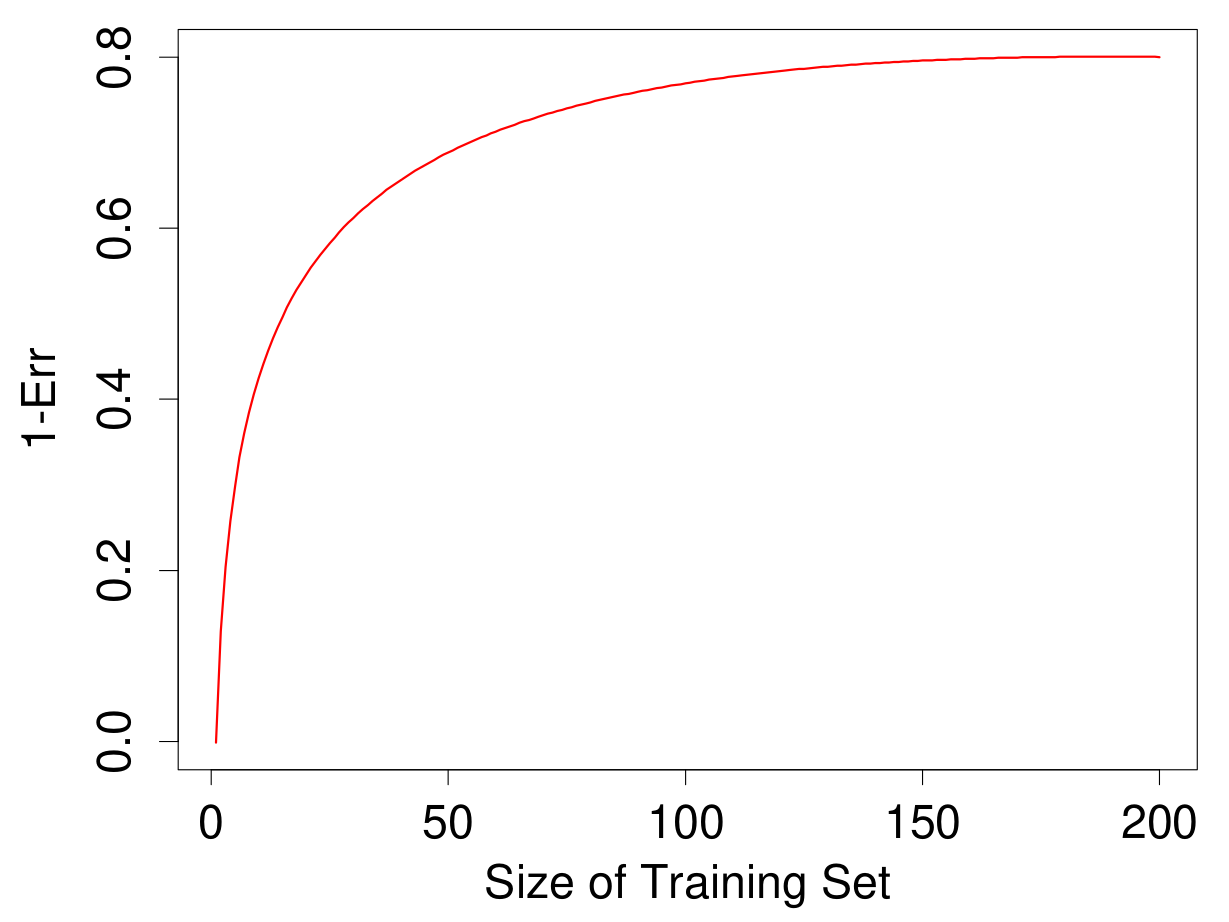
\includegraphics[width=0.8\textwidth]{figures/ml/acc_vs_n.png}
\caption{
Illustration of the decrease in classification error rate
with larger sets of training data \cite{HastieTF09}.
By artificially limiting the available number of data points $n$,
one can create a similar curve to verify that
there is enough statistics in the training data
for the complexity of the model under consideration.
Ideally the curve should reach a clear asymptote before the maximum $n$ is used.
}
\label{fig:additional:misc:enough_data}
\end{figure}

%%%%%%%%%%%%%%%%%%%%%%%%%%%%%%%%%%%%%%%%%%%%%%%%%%%%%%%%
\subsection{Factor Analysis}
\label{additional:misc:factor_ana}
% TODO

%%%%%%%%%%%%%%%%%%%%%%%%%%%%%%%%%%%%%%%%%%%%%%%%%%%%%%%%
\subsection{Optimization and Lagrange Multipliers}
\label{additional:misc:opt}
% TODO

%%%%%%%%%%%%%%%%%%%%%%%%%%%%%%%%%%%%%%%%%%%%%%%%%%%%%%%%
\subsection{Information Theory}
\label{additional:misc:info_theory}
% TODO
% TODO Entropy, significance of bits

%%%%%%%%%%%%%%%%%%%%%%%%%%%%%%%%%%%%%%%%%%%%%%%%%%%%%%%%
\subsection{Modulo Operations}
\label{additional:misc:modulo}

\begin{subequations}\label{eq:additional:misc:modulo}
\begin{align}
\left(A~\text{mod}~C\right)~\text{mod}~C &= A~\text{mod}~C, \label{eq:misc:additional:modulo:basic} \\
\left(A \pm B\right)~\text{mod}~C &= \left(A~\text{mod}~C \pm B~\text{mod}~C\right)~\text{mod}~C, \label{eq:misc:additional:modulo:pm} \\
\left(A \times B\right)~\text{mod}~C &= \left(A~\text{mod}~C \times B~\text{mod}~C\right)~\text{mod}~C, \label{eq:misc:additional:modulo:multiplication} \\
A^{B}~\text{mod}~C &= \left(\left(A~\text{mod}~C\right)^{B}\right)~\text{mod}~C. \label{eq:misc:additional:modulo:exp}
\end{align}
\end{subequations}
